\documentclass[12pt]{article}

\usepackage[pdftex]{graphicx}
\usepackage{cancel}
\usepackage[margin=4cm]{geometry}
\usepackage[hidelinks]{hyperref}
\usepackage{fancyhdr}
\usepackage{amsmath}
\usepackage{amsfonts}
\usepackage{dirtytalk}
\usepackage{parskip}

\newcommand\tab[1][1cm]{\hspace*{#1}}
\newcommand{\HRule}{\rule{\linewidth}{0.5mm}}
\newcommand{\course}{COMS 474}

\setcounter{secnumdepth}{0} % Disable section/subsection numbering
\hyphenpenalty 10000 % Prevent words from being broken over multiple lines
\exhyphenpenalty 10000 % Prevent words from being broken over multiple lines

% Margins
\topmargin=-0.45in
\evensidemargin=0in
\oddsidemargin=0in
\textwidth=6.5in
\textheight=9.0in
\headsep=0.25in
\title{ \course \\\large Homework 6 }
\author{ Haadi Majeed }
\date{Spring 2022}


\pagestyle{fancy}
\fancyhead{}
\fancyfoot{}
\lhead{\course}
\chead{Haadi Majeed}
\rhead{Page \thepage}

\begin{document}
\maketitle
\pagebreak

% Optional TOC
%\tableofcontents
\pagebreak
\section{Problem 1}
 [8 points]\\
Recall that for a two-class \{0, 1\} classification problem with $p$ features \{$X_1, . . . , X_p$\}, logistic regression models have the form
\begin{center}
    \[
        P(Y=1 | X_1, . . . , X_p) = \frac{e^{\beta_0+\beta_1X_1+...+\beta_pX_p}}{1 + e^{\beta_0+\beta_1X_1+...+\beta_pX_p}} \tab P(Y=0 | X_1, . . . , X_p) = \frac{1}{1 + e^{\beta_0+\beta_1X_1+...+\beta_pX_p}}
    \]
\end{center}
For a model with fitted coefficients \{$\beta_0, \beta_1, . . . , \beta_p$\}, what is the boundary between $\hat{Y} = 1$ and $\hat{Y} = 0$? Simply your work as much as possible.


By assigning the equations equal to each other, and since they have identical values in the denominator we can be sitting with $e^{\beta_0+\beta_1X_1+...+\beta_pX_p} = 1$ and we then assign ${X_1, ..., X_P} = 0$ along with $\beta_0 = 0$. We can get the following sequence of equations:
\begin{center}
    \[
        \frac{e^{\beta_0}}{1 + e^{\beta_0}} = \frac{1}{1 + e^{\beta_0}}
    \]
    \[
        \frac{1}{1+1} = \frac{1}{1+1}
    \]
    \[
        \frac{1}{2} = \frac{1}{2}
    \]
\end{center}
Resulting with a boundary of $x = \frac{1}{2}$ where the two functions intersect at.
\pagebreak
\section{Problem 2}
 [15 points (8,2,5)]\\
In this problem you will identify the max margin classifier for the following data set with three samples.
\begin{center}
    \begin{tabular}{ |c|c|c|c| }
        \hline
        Sample \# & $Y$ & $X_1$ & $X_2$ \\
        \hline
        1         & +1  & 0     & 2     \\
        \hline
        2         & -1  & 0     & 0     \\
        \hline
        3         & +1  & -2    & 0     \\
        \hline
    \end{tabular}
\end{center}
You do \underline{not} need to draw a scatter plot of these samples, though it may help you to check your answers to the following questions.
\subsection{A}
What are the set of coefficients \{$\beta_0, \beta_1, \beta_2$\} for the line
\begin{center}
    \[
        \beta_0 + \beta_1X_1 +\beta_2X_2 = 0
    \]
\end{center}
that passes through the two $Y = +1$ samples? Normalize the coefficients so that $\beta_1^2 + \beta_2^2 = 2$ (In lecture we used a different normalization; this is chosen to simplify your work).
\newline
Since there are two $ Y = +1$ samples, we create a system of equations.
\begin{center}
    The first sample:\\ $\beta_1 + \beta_1(0) + \beta_2(2) = 0$\\
    $\beta_0 + 2\beta_2 = 0$\\
    The second sample:\\ $\beta_1 + \beta_1(-2) + \beta_2(0) = 0$\\
    $\beta_0 - 2\beta_1 = 0$\\

    With this, we can determine the following:
    \begin{tabular}{ |c|c|c| }
        \hline
        $\beta_0$ & $\beta_1$ & $\beta_2$ \\
        \hline
        2         & 1         & -1        \\
        \hline
    \end{tabular}\\
    This satisfies the normalization equation resulting with:\\${-1}^2+1^2=2$
\end{center}
\subsection{B}
Confirm whether your coefficients \{$\beta_0, \beta_1, \beta_2$\} of $\beta_0 + \beta_1X_1 +\beta_2X_2$ evaluates positive or negative for the $Y = -1$ sample.


If the evaluation is positive, change your formula so that it evaluates as negative for that sample.

\begin{center}

    The coefficients\\
    \begin{tabular}{ |c|c|c| }
        \hline
        $\beta_0$ & $\beta_1$ & $\beta_2$ \\
        \hline
        2         & 1         & -1        \\
        \hline
    \end{tabular}\\
    We can enter into the formula:\\
    $2 + 1 * 0 + -1 * 0 = 2$\\
    Since it is positive, we can modify all $\beta$ values while still maintaining validity for part A by doing the following:\\$-1 * \{\beta_0, \beta_1, \beta_2\}$
\end{center}

\subsection{C}
Using your results from A and B, guess what the optimal separating line (i.e. the boundary line for the max margin classifier)
\begin{center}
    \[
        \widetilde{\beta_0} + \widetilde{\beta_1}X_1 + \widetilde{\beta_2}X_2 = 0
    \]
\end{center}
is with $\widetilde{\beta_1^2} + \widetilde{\beta_2^2} = 2$.\\
Confirm that using the classifier
\begin{center}
    \[
        \hat{Y}(X_1, X_2) = sign \bigg(\widetilde{\beta_0} + \widetilde{\beta_1}X_1 + \widetilde{\beta_2}X_2 \bigg)
    \]
\end{center}
achieves zero classification error and that all training samples have the same magnitude of $\widetilde{\beta_0} + \widetilde{\beta_1}X_1 + \widetilde{\beta_2}X_2$.


Using properties from \emph{A} and \emph{B} We can fill in the formula
\begin{center}
    \[
        \hat{Y}(X_1, X_2) = - \bigg(\widetilde{2} + \widetilde{1}X_1 - \widetilde{1}X_2 \bigg)
    \]
    When we plug in the values for each of the samples, we get the following:\\
    Sample 1: $-(2+1*0-1*2 = 0)$\\
    Sample 2: $-(2+1*0-1*0 = -2)$\\
    Sample 3: $-(2+1*-2-1*0 = 0)$\\
    Thus we need to adjust the value of $\beta_0$ from $2$ to $1$ in order to get a more equal distribution.\\
    Sample 1: $-(1+1*0-1*2 = 1)$\\
    Sample 2: $-(1+1*0-1*0 = -1)$\\
    Sample 3: $-(1+1*-2-1*0 = 1)$\\
    This modified version now has a correct sign of negative one, and confirms the new classifier with equal magnitudes and zero error.
\end{center}



\pagebreak
\section{Problem 3}
 [24 points (15, 4, 2, 3)]\\
You are working on a two-class \{A,B\} classification problem using two features \{$X_1, X_2$\}. You decide to use QDA. You estimate the mean vectors for each class and find that they are the same,
\begin{center}
    $
        \widehat{\mu_A} = \begin{bmatrix}
            0 \\ 0
        \end{bmatrix}
        \tab
        \widehat{\mu_B} = \begin{bmatrix}
            0 \\ 0
        \end{bmatrix}
    $
\end{center}
When you estimate the covariance matrices, you find they are both diagonal matrices,
\begin{center}
    $
        \widehat{\sum_A} = \begin{bmatrix}
            1 & 0 \\
            0 & 1
        \end{bmatrix}
        \tab
        \widehat{\sum_B} = \begin{bmatrix}
            4 & 0 \\
            0 & 4
        \end{bmatrix}
    $
\end{center}
Lastly, the number of samples for Class \emph{A} and \emph{B} are the same, so $\widehat{\pi_A} = \frac{1}{2} = \widehat{\pi_B}$.

\subsection{A}
What is the equation for the QDA decision boundary for this problem? Simplify it as much as possible.


\subsection{B}
Sketch a plot by hand showing the boundary. Indicate for what region(s) $\hat{Y} = A$ and for what region(s) $\hat{Y} = B$


\subsection{C}
What would the prediction be for the mean value of both conditional distributions, $\begin{bmatrix}0 \\ 0\end{bmatrix}$? What would the prediction be for the point $\begin{bmatrix}3 \\ -3\end{bmatrix}$?


\subsection{D}
Suppose we had a third class \emph{C}, also centered at the origin and with a diagonal covariance matrix,
\begin{center}
    $\widehat{\mu_C} = \begin{bmatrix}
            0 \\
            0
        \end{bmatrix}
        \tab
        \widehat{\sum_C} = \begin{bmatrix}
            9 & 0 \\
            0 & 9
        \end{bmatrix}
    $
\end{center}
and that all classes had equal priors, $\pi_A = \pi_B = \pi_C = \frac{1}{3}$.\\
Sketch a plot similar to B, of the decision regions for this problem with three classes (e.g. make it clear on the plot what region has $\hat{Y} = A$, what region has $\hat{Y} = B$, and what region has $\hat{Y} = C$). You do not need to do calculations, but extrapolate from what you just observed for the two class problem.\\
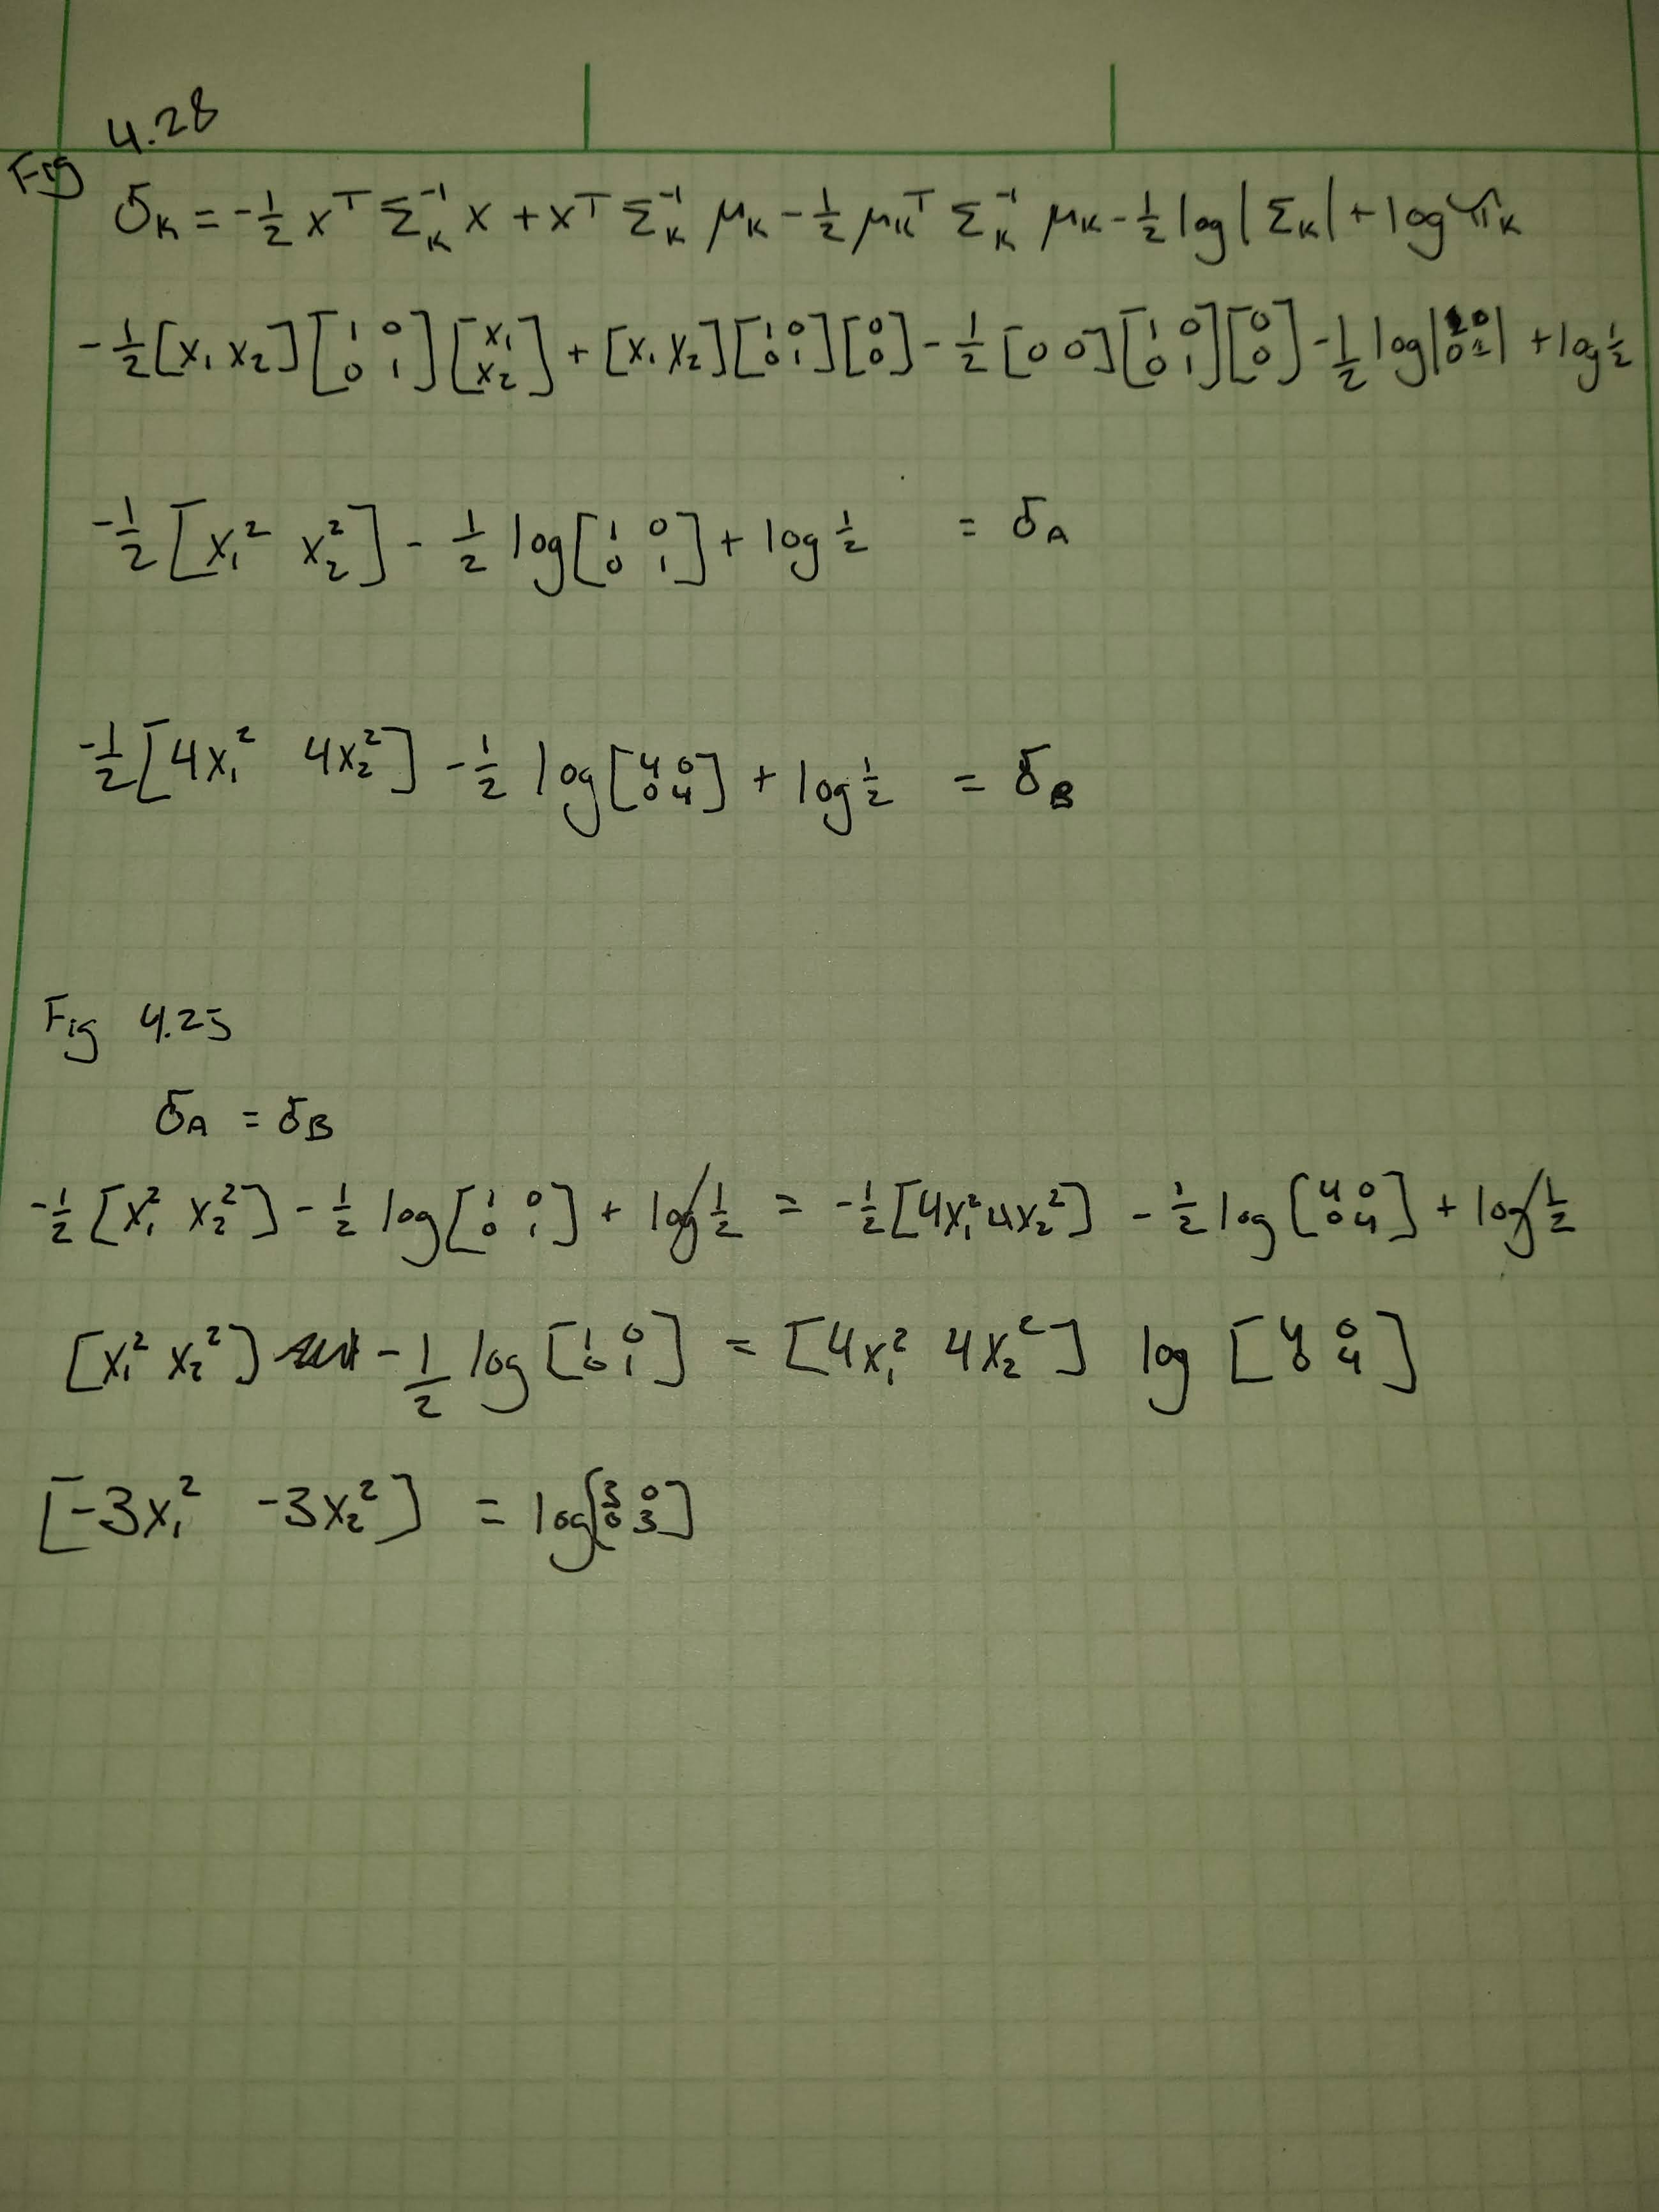
\includegraphics[width=1\textwidth]{q3_progress.jpg}\\
I was not able to make much progress past this point, I just ended up getting answers that seemed more and more wrong :$|$ .
%--/Paper--
\end{document}